\documentclass[a4paper,11pt]{article}


\usepackage{amsmath,amsfonts,amsthm,a4wide}
\usepackage{graphicx}
\usepackage[super]{nth}
\usepackage{mathtools}


\begin{document}
\begin{center}
University of Toronto at Scarborough\\[0.1in]
{\bf CSCC73H3 Algorithm Design and Analysis, FALL 2018} \\[0.1in]
{\large{\bf Assignment No.5.Q1: Dynamic Programming and Network Flow}}\\[0.1in]
{\bf DUE:} November 15, 2018, at 11:59 pm
\end{center}


\vspace{0.1in}
\noindent
{\bf Student ID:} 1005642654 \\[0.15in]
{\bf Student Name:} KyooSik Lee
\vspace{0.3in}

\vspace{0.3in}
\begin{enumerate}

\item {\bf Description}

The maximum $s$, $t$-flow in G has value $k$. Therefore there are k disjoint path from $s$ to $t$. Then say each path is consisted of nodes $v_1, v_2, ... v_n$.
Then make a $pulse$ operation to find where it is disconnected. So first make a $pulse$ on the $v_\frac{n}{2}$. If this signal sends that it is not connected, we look for first half ($v_1, v_2, ... v_\frac{n}{2}$). If this is not, then look for the second half. This is similar to binary searching. If we find node $v_i$ such that $v_1, v_2, ... v_i$ is connected as $v_{i+1},...,v_n$ is not connected, we know that the nodes from  $v_1, v_2, ... v_i$ is connected nodes, and $v_{i+1},...,v_n$ is not. Do the algorithm to the next disjoint path.

{\bf Complexity}

For each of the path, finding the node $v_i$ takes $O(log n)$ time complexity, given that the number of node in that path is at most $n$. And we have $k$ disjoint path. Therefore the complexity is $O(k log n)$.

\pagebreak
\item {\bf Description}

First, use Fold-Fulkerson algorithm to make a max flow out of the flow network $G$. Then, set $A$ consisted of nodes that are reachable from source by residual graph is $upstream$. And set $B$ consisted of nodes that are reachable to sink by residual graph is $downstream$. Any node else is $central$.

{\bf Complexity}

The complexity of my algorithm is same as the time required to compute a single maximum flow. We just need to find $A$ by bfs starting from $s$. And we just need to find $B$ by bfs starting from $t$ with reversed residual graph.


{\bf Proof}

Let's say that the set $S$ contains $s$ and $a_1, a_2, ... a_i$. Then at the residual graph, if we consider $A$ and $V-A$

\begin{figure}[hbt]
	\centering
	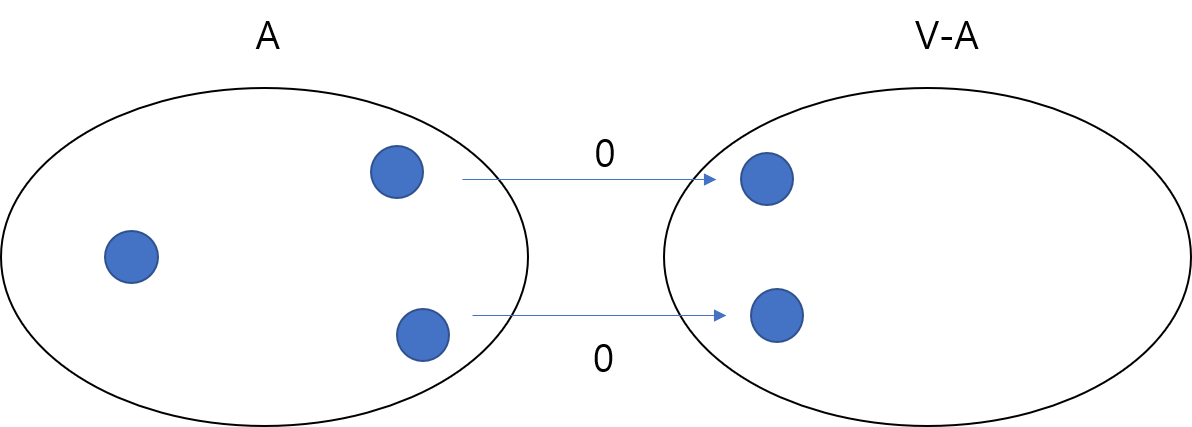
\includegraphics[scale=0.4]{figure1.png}
	\caption{A and V-A}
\end{figure}

Then the edges from $A$ to $V-A$ will be 0, by the definition of $A$.
And there is no set that has less nodes than $A$ and still be minimum cut.
Also, every minimum cut has to include nodes in $A$.
If not, say $A'$ is the minimum cut without one node in $A$. then the min-cut capacity will increase by the residual graph edge from $A'$ to that one node. Therefore every min cut has to include nodes in $A$. 
Similary, every $downstream$ should include $B$. 
Therefore the $upstream$ is $A$ and $downstream$ is $B$, and $central$ is $V-A-B$.


\end{enumerate}







\end{document}

\iffalse
\begin{figure}[hbt]
	\centering
	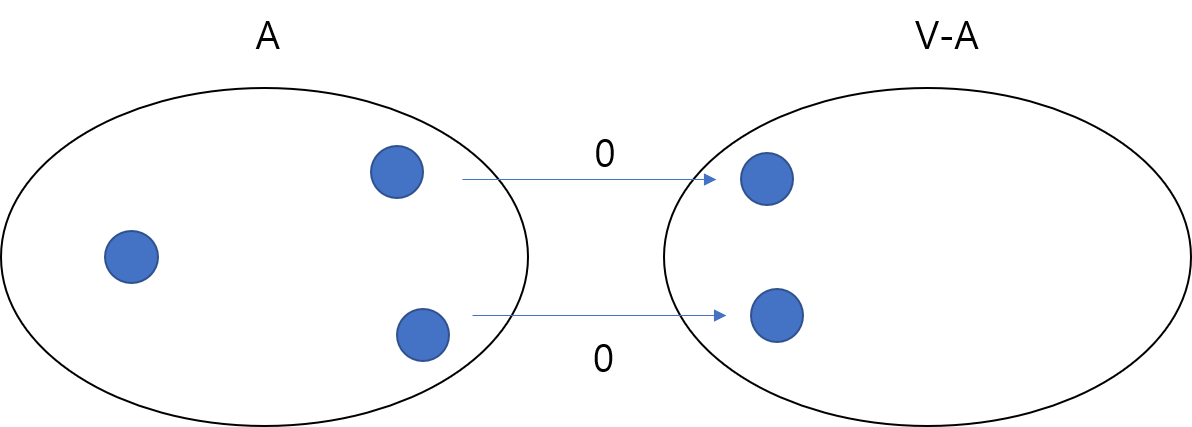
\includegraphics[scale=0.4]{figure1.png}
	\caption{Basic Tree}
\end{figure}
\fi
